\documentclass[american,twocolumn]{bmcart}
\makeatletter
%%%%%%%%%%%%%%%%%%%%%%%%%%%%%% User specified LaTeX commands.
\usepackage{paperBMC_preamble}

\begin{document}
\begin{frontmatter}
\begin{fmbox}
\dochead{Research}

\title{Fast parallel algorithm to reduce protein folding trajectories}

\maketitle
\author[
   addressref={aff1},                   % id's of addresses, e.g. {aff1,aff2}   
   email={lgarreta@agrosavia.co}   % email address
]{\inits{LG}\fnm{Luis} \snm{Garreta}}
\author[
   addressref={aff2},
   email={mmartinez@ebi.ac.uk}
]{\inits{MM}\fnm{Mauricio} \snm{Martinez}}
\author[
   addressref={aff3},
   email={nediaz@unicauca.edu.co}
]{\inits{ND}\fnm{Néstor A} \snm{Díaz}}
\author[
   addressref={aff4},
   corref={aff4},                       % id of corresponding address, if any
   email={pedro.moreno@correounivalle.edu.co}
]{\inits{PM}\fnm{Pedro A} \snm{Moreno}}

%%%%%%%%%%%%%%%%%%%%%%%%%%%%%%%%%%%%%%%%%%%%%%%%%%%%%%%%
\address[id=aff1]{%                           % unique id
  \orgname{Corporaci\'{o}n Colombiana de Investigaci\'{o}n Agropecuaria - AGROSAVIA, CI Tibaitat\'{a},  Kil\'{o}metro 14, V\'{i}a a Mosquera, 250047, Colombia}, % university, etc
  %\street{},                     %
  %\postcode{}                                % post or zip code
  \city{Santiago de Cali},                              % city
  \cny{Colombia}                                    % country
}
\address[id=aff2]{%
  \orgname{The European Bioinformatics Institute (EMBL-EBI)},
  %\street{D\"{u}sternbrooker Weg 20},
  %\postcode{24105}
  \city{Hinxton, Cambridgeshire},
  \cny{UK}
}
\address[id=aff3]{%                           % unique id
  \orgname{Facultad de Ingeniería Electrónica y Telecomunicaciones,  Universidad del Cauca}, % university, etc
  %\street{},                     %
  %\postcode{}                                % post or zip code
  \city{Popayán},                              % city
  \cny{Colombia}                                    % country
}
\address[id=aff4]{%                           % unique id
  \orgname{Escuela de Ingeniería de Sistemas y Computación, Universidad del Valle}, % university, etc
  %\street{},                     %
  %\postcode{}                                % post or zip code
  \city{Santiago de Cali},                              % city
  \cny{Colombia}                                    % country
}

\begin{artnotes}
\note[id=n1]{Equal contributor} % note, connected to author
\end{artnotes}


%\end{fmbox}% comment this for two column layout
\begin{abstractbox}
\begin{abstract}
\parttitle{Background} The simulations are one of the most important tools for studying and understanding the underlying mechanisms of the protein folding process. Protein folding simulations have experienced substantial progress in the last years, they are performed using diverse technologies and they are reaching the microseconds and greater timescales, which generates very long trajectories. As a result, the analysis of these trajectories entails to complications and is necessary to create tools to simplify them, so that both the main events and the temporal order in which they occur are preserved.

\parttitle{Results} We present an algorithm to reduce long protein folding trajectories in a fast and parallel way. The algorithm divides a trajectory into segments to be processed in parallel, and from each segment selects the most representative conformations using a rapid clustering strategy, which takes advantage of the temporal order of the conformations to compare them locally, avoiding an all-versus-all comparison. The algorithm reduces a trajectory in a high percentage, preserving both the patterns and the structure obtained by other more complex reduction techniques. In addition, its performance is close to that shown by other efficient reduction techniques, and this performance is improved when executed in parallel using more than one core.

\parttitle{Conclusions} The developed algorithm quickly reduces a protein folding trajectory by selecting its most representative conformations and thus preserving both its structure and its temporal order. The reduced trajectories can be used as input for more complex analysis techniques and even for other reduction techniques that become impractical when faced with long folding trajectories. The algorithm is fast and is designed to run in parallel on conventional PCs with multi-core technology, which are present in most typical research laboratories.
\end{abstract}
\begin{keyword}
\kwd{Protein folding simulations}
\kwd{Protein structure comparison}
\kwd{Protein structure clustering}
\end{keyword}

\end{abstractbox}
\end{fmbox}% uncomment this for two column layout 
\end{frontmatter}

\section*{Background}

We present a parallel algorithm to reduce protein folding trajectories which quickly obtains representative conformations, conserving both their three-dimensional structure (3D) and their temporal order. Proteins play a fundamental role in all living beings, but to be functional, they must fold from their linear amino acid (AA) sequence to a unique 3D or native state, which is known as the protein folding process. Understanding the mechanisms and rules of this process has been one of the most pursued objectives of computational biology, and an important theoretical tool to study it has been the simulations of protein folding. These simulations generate folding trajectories (Figure \ref{fig:Folding-Trajectory}), which describe the sequence of states that proteins follow as a function of time during their folding process.

\begin{figure}[th]
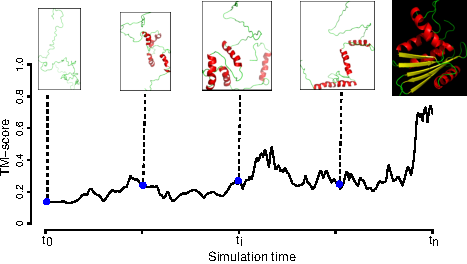
\includegraphics[bb=0bp 0bp 224bp 127bp]{images/trajectory-description-2RN2-pdbs}

\caption{\csentence{Protein folding trajectory.} The evolution of the folding is measured at each step by comparing the structure at time $t_i$ to the native structure (black image background) using a structure comparison metric, in this work we use the TM-Score (see Methods). X-axis: Simulation time from $t_0$ to $t_n$. Y-axis: TM-score value, from 0 (different) to 1 (similar).\label{fig:Folding-Trajectory}}
\end{figure}

Folding simulations mainly use the molecular dynamics (DM) method, which due to its computational cost is limited to small proteins (<100 AA) and very short times (picoseconds or microseconds). However, technological innovations have allowed significant advances in these simulations, both on time scales and technology to execute them. In 2011, using the Anton supercomputer, specially designed for protein folding \cite{Shaw2008}, full simulations of 12 proteins were published, several on the order of milliseconds \cite{Shaw2011}. And more recently, in 2016, the Anton 2 supercomputer became operational \cite{Shaw2014}, being up to ten times faster than its predecessor Anton. As an economic alternative, in 2014 graphic processing units (GPU) were used to simulate, on the order of microseconds, the folding of 17 proteins \cite{Nguyen2014}. And years earlier, in 2007, the \textquotedbl{}folding@home\textquotedbl{} distributed computing platform utilized as many as 250,000 PCs, voluntarily available around the world, to simulate on the order of microseconds the folding of the villin-headpiece protein \cite{Larson2009}.

These innovations show significant progress in protein folding simulations, both on time scales and technology to execute them, and as a result the generation of trajectories with millions of conformations. But due to their large number of conformations, their processing and analysis in conventional PCs is computationally expensive, and new algorithms are needed to efficiently simplify them, seeking to preserve as much information as possible.

Two approaches used to reduce these simulations have been the dimensionality reduction \cite{Duan2013} and clustering \cite{Peng2018}. In the dimensionality reduction approach, conformations are transformed into reduced sets of variables that represent them as well as possible. Here, both linear and non-linear techniques have been used (e.g. principal component analysis (PCA) and multidimensional scaling \cite{RajanSchulten10}, Isomap \cite{Das2006}, diffusion maps \cite{Kim2015}). However, many of these techniques, instead of reducing a trajectory, analyze it, losing the structural information of the conformations (Figure \ref{fig:lost-info-dimensionality}, top) and making the results explainable only when observed together. In addition, many of these techniques require pairwise comparisons, which are computationally expensive when trajectories are very large.

In the clustering approach, the conformations are assigned to groups that share similar characteristics (e.g., similarity with the native structure), and from each group an average representative or its general characteristics can be taken. Here, hierarchical and partitioned groupings have been used (e.g., k-means \cite{Doerr2017}, link \cite{Shao2007}). However, the groups lose their temporal order since they can include conformations that occur in very distant times (Figure \ref{fig:lost-info-dimensionality}, bottom). And also they require pairwise comparisons, which are computationally expensive when trajectories are very large.

\begin{figure}[th]
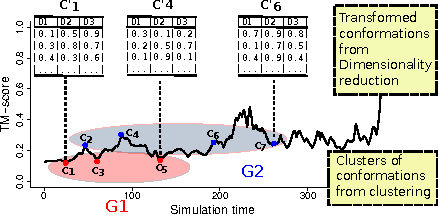
\includegraphics[bb=0bp 0bp 210bp 104bp,scale=1.05]{images/2RN2-trajectory-weakness}

\caption{\csentence{Loss of information in dimensionality reduction and clustering.} The dimensionality reduction (above) transforms the conformations (c1, c2 and c3) into a new set of values (c'1, c'2 and, c'3), but their structural information is lost. While the clustering (bottom) forms two groups (G1 and G2), but their temporal order is lost since they contain conformations that overlap in time (c2, c3, c4, c5). \label{fig:lost-info-dimensionality}}
\end{figure}

To reduce a folding trajectory, the proposed algorithm divides the path into segments that are processed in parallel. For each segment, characteristic events are quickly extracted using the rapid clustering strategy of Hobohm and Sander (1992) adapted for protein folding trajectories; and from these results, the most representative events are selected by a strategy of k-medoids \cite{Kaufman1990}.The results of each segment are joined to form the reduced trajectory with the most representative conformations of the original trajectory, while retaining both its 3D representation as their temporal order.

The algorithm is implemented in the R language, except the function for pairwise structure comparison, the TM-score \cite{Zhang2004}, which is the function executed more times and that is implemented in the Fortran language.

\section*{Methods}

\subsection*{Datasets of protein folding trajectories}

We used the folding trajectories of three proteins taken from different simulation projects. First, the trajectory of the trp-cage protein, simulated with molecular dynamics (MD) using the Anton supercomputer \cite{Shaw2011}, with a simulation time of 208 \us, a 200 \ps~time step, and 1044001 conformations. Second, the trajectory of the villin-headpiece protein, also simulated with DM using the folding@home distributed platform \cite{PandeEnsign07}, with a simulation time of 8 \us, a 50 \ps~ time step, and 15201 conformations. And third, the trajectory of the ribonuclease H protein, simulated with the Probabilistic Roadmap Method using the Parasol folding server \cite{Amato2010}, with 429 folding steps (instead of time steps, see below) each corresponding to 429 conformations. 

\subsection*{Time steps and Folding steps}

A time step in MD trajectories is the time length at which conformations are sampled or evaluated during the simulation. While a folding step, in the PRM and in the reduced trajectories produced by our algorithm, represents the most likely conformation occurring during a time interval or from a set of likely candidate conformations.

\subsection*{Pairwise comparison of protein structures using the TM-score \label{sec:Comparing-Structures}}

In this work, we used the TM-score metric for pairwise comparison of protein structures \cite{Zhang2004}. This metric is used in both the proposed algorithm and in the techniques for reduction of protein folding used to compare its results. The TM-score is more sensitive to the global topology than local variations, and so it estimates the pairwise similarity of protein structures much more accurately than the Root Mean Square-Deviation (RMSD), a common metric used for the same purpose. The TM-score ranges from 0 to 1, where 1 is a perfect match. Based on statistics \cite{zhang2010}, a TM-Score lower than 0.17 indicates two random structures with no relation of similarity, and a TM-Score higher than 0.5 indicates that the structures have a degree of similarity that is not given by chance.

\subsection*{Other techniques for protein folding reduction \label{subsec:Techniques-for-reduction}}

nMDS and clustering techniques were used to get the intrinsic information from both the original and two reduced trajectories of the villin-headpiece protein \cite{Larson2009}, and then compare them (See results).

nMDS reductions were carried out using the R-function monoMDS \cite{Oksanen2019}, taking as input the dissimilarity matrix obtained from the pairwise comparison of all the protein conformations of the folding trajectory. And, the complete-linkage clustering reductions were carried out using the R-function hclust \cite{RCoreTeam2018}, taking as input a matrix with the first two principal components from a PCA analysis. This PCA analysis was carried out using the R-function pca.xyz \cite{Grant2006}, taking as input a matrix with the 3D coordinates of the $C\alpha$ atoms of all the protein conformations of the folding trajectory.

The reduced trajectories were calculated with the proposed algorithm from the villin-headpiece trajectory with 15201 conformations. The first with 7197 conformations (reduced by 52\%), and the second with 2258 conformations (reduced by 80\%). 

\section*{Implementation}

The proposed algorithm reduces a trajectory of protein folding in three steps: partitioning, extraction, and selection. The first step runs only once, while the other two runs several times independently, allowing them to run in parallel. Each step involves a strategy to improve the efficiency of the algorithm when working with large protein folding trajectories. Figure \ref{fig:Algorithm-Description} shows the overview of the algorithm and the steps are given below.

\begin{figure}[th]
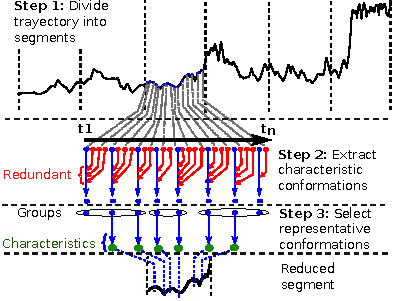
\includegraphics[scale=1.2]{images/algorithm-description-general}

\caption{\csentence{Overview of the proposed algorithm.} Step 1: Divide the trajectory into segments (vertical dashed lines) and reduce each individually. Each segment has n conformations from time $t_1$ to $t_n$. Step 2: For each segment, extract characteristic conformations (blue dots) and remove redundant ones (red dots). Stage 3: Select the most representatives from the previous conformations. \label{fig:Algorithm-Description}}
\end{figure}


\subsection*{Step 1: Partitioning}

Divide the trajectory into segments to reduce them locally and in parallel (dotted vertical lines, Figure \ref{fig:Algorithm-Description}). This is carried out by dividing the trajectory from the start to the end in segments with \emph{N} conformations each, where \emph{N} is an input parameter. Local reductions allow to focus on the particular characteristics of each segment that will determine the global characteristics of the trajectory. And parallel reductions allow to improve the algorithm efficiency when it runs on machines with more than one processor (e.g. multi-core computers) (Figura \ref{fig:Algorithm-Parallel}).

\begin{figure}[th]
\begin{centering}
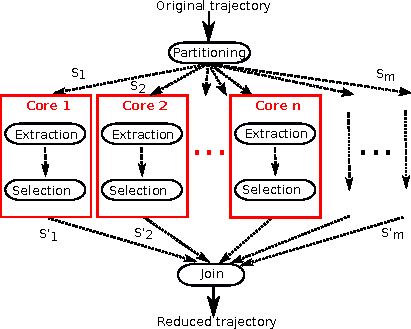
\includegraphics{images/algorithm-description-parallel}
\par\end{centering}
\caption{\csentence{Parallel processing of trajectory segments.} The trajectory is divided into m segments (S1, ..., Sm), and each segment is processed separately and in parallel on a machine with n processing cores. The results of the extraction and selection steps (S1 ', ..., Sm') are independent of each other and join to form the reduced trajectory. \label{fig:Algorithm-Parallel}}
\end{figure}


\subsection*{Stage 2: Extraction}

Quickly extract the characteristic conformations of each segment and eliminate the redundant ones. This is carried out efficiently by means of a rapid clustering approach that performs relatively few pairwise comparisons and, instead of grouping similar conformations of a segment, extracts the most dissimilar ones.

Here, we improved the fast clustering algorithm of Hobohm and Sander (1992) to work with a trajectory segment and exploit the implicit order of its conformations given by its simulation time (black horizontal line, Figure \ref{fig:Algorithm-Description}). The algorithm selects the initial conformation at time $t_1$ as the first characteristic. Then, the algorithm compares the previous characteristic with the following conformation. If dissimilar, then the conformation becomes a new characteristic, otherwise, the conformation is redundant and is removed (red dots, Figure \ref{fig:Algorithm-Description}). The process continues with the rest of conformations until finishing in the final one at time $t_n$, thus producing the set of representative characteristics of the segment (green dots, Figure \ref{fig:Algorithm-Description})

\subsection*{Step 3: Selection}

Take the conformations of previously extracted characteristics and cluster them to select the most representative characteristics. To find these rep$\text{\ensuremath{\text{\ensuremath{\text{}}}}}$resentatives, the algorithm uses a k-medoids strategy (PAM algorithm \cite{Kaufman1990}) that calculates the k conformations (medoids) whose average difference between all the other members of the group is minimal.

However, the PAM algorithm needs as input the dissimilarity matrix with the pairwise comparison of all-versus-all conformations of the trajectory segment, which is an intensive computational task when the number of conformations is very large. But, this task is feasible to perform since the algorithm is working here with a reduced set of characteristic conformations (previous step) of a trajectory segment and not of the complete trajectory.


\section*{Results and Discussion}

Three tests were carried out to evaluate the capacity and performance of the proposed algorithm: first, reduction of three trajectories using the proposed algorithm; second, comparison of the intrinsic information preserved by the reductions from both the proposed algorithm and two other folding reduction techniques; and third a performance comparison.

\subsection*{Reduction of protein folding trajectories}

Figure \ref{fig:Trajectory-Results} shows the TM-score plots of the reduced trajectories produced by the proposed algorithm. It can be seen from the plots that the algorithm try to find the most representative conformations from their original trajectories, conserving two fundamental properties: the structure and the temporal ordering of the original conformations. Other folding reduction methods lose these properties in their reductions, as we will see in the next section.

As a result, these reduced trajectories become a summary of the original ones and can be used as inputs for more complex analyzes, or even for other reduction methods that require pairwise comparisons and become impractical for large trajectories.

\begin{figure*}[!t]
\begin{raggedright}
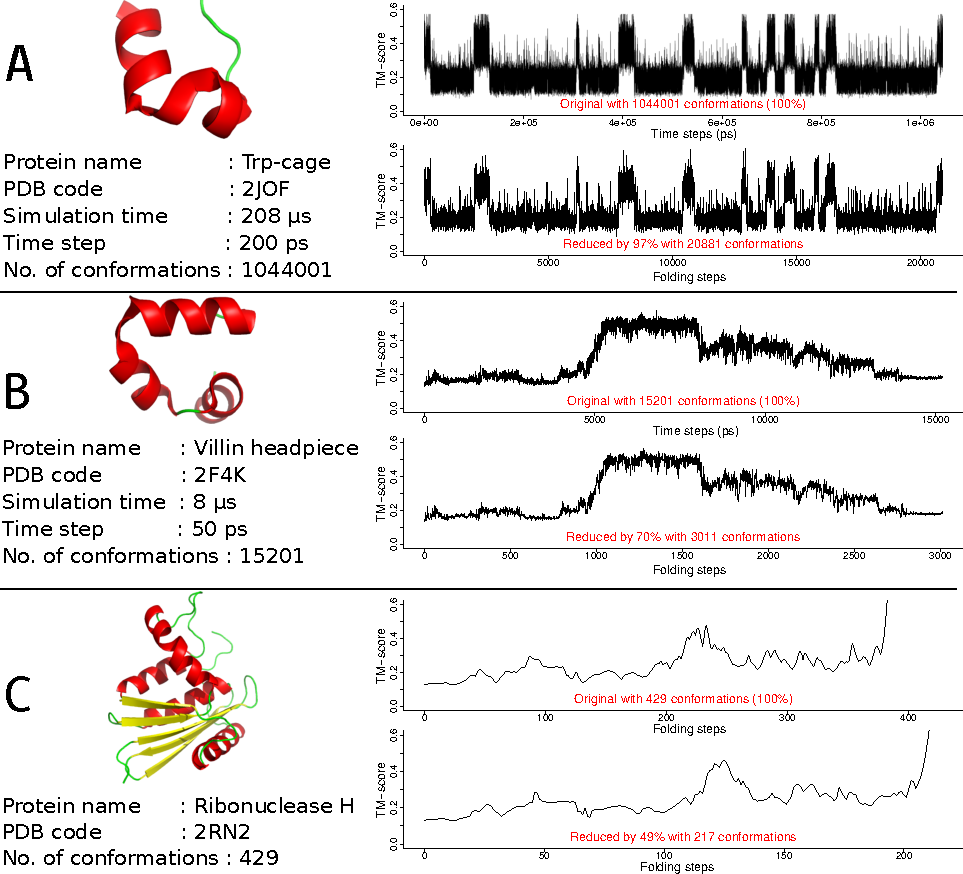
\includegraphics{images/path-comparisons}
\par\end{raggedright}
\caption{\csentence{Plots of the TM-score values for the original and reduced trajectories.} Protein and simulation details on the left. Trajectories on the right: original (upper part), and reduced (lower part). (A) Trajectory of trp-cage protein,  reduced by 98\%, from 1044001 to 20881 conformations. (B) Trajectory of the villin-headpiece protein, reduced by 80\%, from 15201 to 3011 conformations. (C) Trajectory of ribonuclease H protein, reduced by 49\%, from 429 to 217 conformations.\label{fig:Trajectory-Results}}
\end{figure*}


\subsection*{Comparison with other methods \label{sec:Comparing-other-methods}}

Here, we compared how the intrinsic information captured by other folding reductions techniques from a folding trajectory is also preserved in the reductions produced by the proposed algorithm. First, two reduced trajectories were computed from the original trajectory of the villin-headpiece protein using the proposed algorithm (Figure 6), and then the intrinsic information was computed on these trajectories using nMDS and clustering reductions (Figure 7) (see Methods for the details of the trajectory and techniques). 

As it can be seen from the Figure 7, the pattern of circles of points from nMDS, and the structure of three groups from clustering, repeat in both the original and the reduced trajectories. This shows that the reductions produced by the proposed algorithm largely preserve the intrinsic information observed in the original trajectory. Furthermore, the proposed algorithm has several advantages. First, it avoids the calculation of the dissimilarity matrix as it is done by nMDS and clustering, that is a computationally expensive task for medium to large trajectories. Second, its reductions are a set of protein conformations, contrary to reduced transformations as the produced with other techniques as nMDS, PCA, Isomap or diffusion maps \cite{RajanSchulten10,Duan2014,Kim2015} that lose structural information and that can only be interpreted when viewed together. And third, temporal ordering of conformations is conserved, contrary to clustering methods \cite{Peng2018} that merge configurations from different simulation times into clusters.

\begin{figure}[!th]
\begin{raggedright}
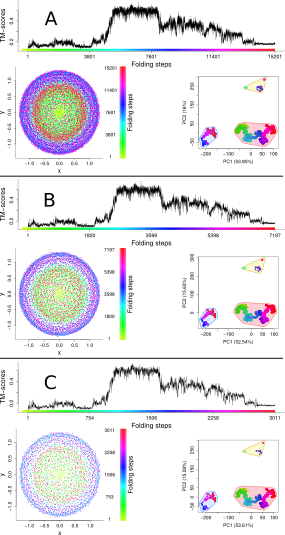
\includegraphics{images/paths-intrinsic-info}
\par\end{raggedright}
\caption{\csentence{Intrinsic information is preserved in the reductions.} Intrinsic information captured from the original trajectory of the villin-headpiece protein is largely preserved in the reduced trajectories produced by our algorithm. TM-score plot, nMDS pattern and clustering groups at the top, bottom left, and bottom right of each figure. (A) Original trajectory (B and C) Reduced trajectories by 52\%. and 80\%, respectively. The nMDS produces a set of circular patterns associated with conformations occurring in different times of the simulation, while clustering produces a structure of three clusters associated with the first two principal components of the $C\alpha$ atoms of the conformations. \label{fig:Comparaciones-PCA-nMDS}}
\end{figure}


\subsection*{Algorithm performance}

The performance of the proposed algorithm was tested in two cases: first, a runtime comparison with other three typical techniques for folding reduction: nMDS, clustering, and PCA; and second, a parallel comparison, running the algorithm with several cores (Figure \ref{fig:Performance-methods}). For both tests, the trajectory corresponds to the first 100k conformations from the full trajectory of the trp-cage protein, described above in datasets section. 

For the comparison between techniques (Figure \ref{fig:Performance-methods}.A), several subtrajectories of different lengths were reduced by all the techniques. PCA showed the most efficient runtimes followed by our proposed algorithm FR, contrary to nMDS and clustering that becomes impractical when faced with short to medium trajectories. However, the proposed algorithm has the advantage to easily run in parallel, contrary to the other techniques, and when it runs using two cores, its runtime is reduced by half and becomes faster than PCA. (FR2, black dashed line).

\begin{figure}[th]
\begin{centering}
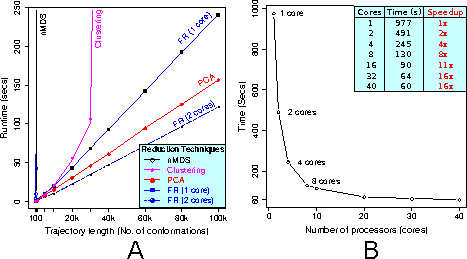
\includegraphics{images/performance-times}
\par\end{centering}
\caption{\csentence{Performance of the algorithm.} (A) Runtime comparisons for four folding reduction techniques: nMDS, clustering, PCA, and our algorithm FR (running with one and two cores). PCA is the most efficient algorithm followed by our algorithm FR with one core, but when it runs with two cores, its runtime is reduced by half, being more efficient than PCA.  (B) Evaluation of the algorithm paralellization. When the number of processing cores is multiplied by two, the processing time reduces by half with a quasi-linear speedup that maintains for up to \textasciitilde{}8 cores (8x). \label{fig:Performance-methods}\protect \\
}
\end{figure}

To test how the parallelization improves the algorithm performance, the full dataset of 100k conformations was reduced by the algorithm using different number of cores. The runtimes are shown in the Figure \ref{fig:Performance-methods}.B, where it is notable a good speedup that reduces the time by half every time the number of cores is duplicated. This speedup maintains for up to \textasciitilde{}8 cores, and then it reduces to the minimum after \textasciitilde{}30 cores.

These results show that the algorithm has a good performance when compared with the other techniques, and this performance improves more when it is run in parallel using more than one core. As a consequence, the speedup of the algorithm scale quasi-linearly with the number of processing cores, almost until 8x, and with 32 cores the algorithm still achieves a speedup of 16x. Now, considering that multi-core technology is quite commonplace for even desktop computers, the proposed algorithm has the capacity to take advantage of this technology to reduce large protein folding trajectories in a fast parallel manner, with runtimes closer or better than other techniques commonly used for this task.

\section*{Conclusions}

Although the progress in long timescale simulations of protein folding has enabled the generation of large folding trajectories, the new challenge is in their analysis, but due to the millions of conformations they can contain, their processing and analysis becomes difficult or impractical. 

Here, we have proposed a fast and parallel algorithm to simplify large protein folding trajectories. The algorithm reduces a trajectory by splitting it into segments and then reducing each in parallel using a fast clustering strategy which avoids the pairwise comparison of all structures. 

According to the results, the algorithm can achieve resumed trajectories with high compression of data and preserving their main conformations, what was confirmed when patterns and clusters produced by other folding reduction techniques were also observed in the algorithm reductions. Furthermore, the algorithm outperformed the performance of the other techniques, apart from the PCA technique. However if the algorithm uses additional processing cores, it outperforms all the other techniques at larger values. 

Nevertheless, the reductions produced by the proposed algorithm are limited to create a summary of the main events of a protein folding trajectory without performing any kind of analysis, as other techniques do. But, these summarized trajectories can be used as input to these and other techniques that serve the same purpose and which were not designed to handle large protein folding trajectories.

\bibliographystyle{bmc_mathphys}
\bibliography{paperBMC_references}

\begin{backmatter}

\end{backmatter}
\end{document}
\end{document}
